\documentclass{beamer}

\usepackage[latin1]{inputenc}
\usepackage[ngerman]{babel}
\usepackage{setspace}
\usepackage{amssymb}
\usepackage{amsmath}
\usepackage{hyperref}
\usepackage{pgf}
\usepackage{graphicx}

\beamertemplatenavigationsymbolsempty
\author[F. Loewe]{
  \leftline{\textbf{Projektpartner}: Paul Thurner}
  \leftline{\textbf{Betreuer}: Goeran Kauermann}
  \leftline{\textbf{Referent}: Felix Loewe}
}
\title[Internationaler Waffenhandel]{Internationaler Waffenhandel}
\subtitle{Die Anwendung neuer Verfahren der statistischen Netzwerkanalyse}
\institute[\textbf{LMU} -- Insitut f�r Statistik]{Ludwig-Maximilians-Universit�t M�nchen \\ Institut f�r Statistik}
\logo{\pgfimage[width=2cm,height=2cm]{lmu_logo}}
%\titlegraphic{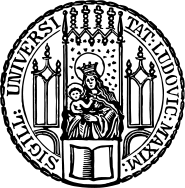
\includegraphics[width=1cm,height=1cm]{lmu_logo}}			
\date{\today}
\usetheme{Madrid}
\colorlet{beamer@blendedblue}{green!40!black}
\bibliographystyle{plain}

\begin{document}

%%%%%%%%%%%%%%%%%%%%%%%%%%%% Titel %%%%%%%%%%%%%%%%%%%%%%%%%%%%%%%
\begin{frame}
\maketitle	
\end{frame}

%%%%%%%%%%%%%%%%%%%%%%%%%%%Inhaltsverzeichnis%%%%%%%%%%%%%%%%%%%%%%%%%%%%
\begin{frame}
	\tableofcontents
\end{frame}

%%%%%%%%%%%%%%%%%%%%%%%%Einleitung%%%%%%%%%%%%%%%%%%%%%%%%
\section{Einleitung}
\begin{frame}
	\frametitle{Was ist ein Netzwerk?}
\end{frame}

%%%%%%%%%%%%%%%%%%%Einf�hrung in die Graphentheorie%%%%%%%
\section{Einf�hrung in die Graphentheorie}
\begin{frame}
	\frametitle{Einf�hrung in die Graphentheorie}
\end{frame}

%%%%%%%%%%%%%%%%%%%%Datensituation%%%%%%%%%%%%%%%%%%%%%%%%
\section{Datensituation}
\begin{frame}
	\frametitle{Datensituation}
\end{frame}

%%%%%%%%%%%%%%%%%Deskriptive Analyse%%%%%%%%%%%%%%%%%%%%%%
\section{Deskriptive Analyse}
\subsection{Netzwerkma�zahlen}
\begin{frame}
	\frametitle{Netzwerkma�zahlen}
\end{frame}
\subsection{Degree-Sequenz}
\begin{frame}
	\frametitle{Degree-Sequenz}
\end{frame}
\subsection{zentrale Akteure}
\begin{frame}
	\frametitle{zentrale Akteure}
\end{frame}
\subsection{Visualisierungen}
\begin{frame}
	\frametitle{Visualisierungen}
\end{frame}

%%%%%%%%%%%%%%%inferentielle Analyse%%%%%%%%%%%%%%%%%%%%
\section{Inferentielle Analyse}
\subsection{ERGM - Exponential Random Graph Model}
\begin{frame}
	\frametitle{ERGM - Exponential Random Graph Model}
\end{frame}
\subsubsection{Simulation von Zufallsgraphen}
\begin{frame}
	\frametitle{Simulation von Zufallsgraphen}
\end{frame}
\subsubsection{Sch�tzung der Modellparameter}
\begin{frame}
	\frametitle{Sch�tzung der Modellparameter}
\end{frame}
\subsection{Anwendung des ERGM}
\begin{frame}
	\frametitle{Anwendung des ERGM}
\end{frame}
\subsection{Vergleich mit Gro�waffenhandel}
\begin{frame}
	\frametitle{Vergleich mit Gro�waffenhandel}
\end{frame}

%%%%%%%%%%%%%%%%Fazit%%%%%%%%%%%%%%%%
\section{Fazit}
\begin{frame}
	\frametitle{Fazit}
\end{frame}
\end{document}